
\chapter{Ugeopgave 11}
\label{cha:ugeopgave-11}

\section{Part 1}

I \textit{B-splines} er der ingen relation mellem graden af kurven og antallet af kontrolpunkter, men antallet af kontrolpunkter skal v�re st�rre eller lig med ordenen af kurven, hvorimod \texttt{Bezier} kurver bruger ordenen+1 kontrolpunkter.

\texttt{B-spline} kurver af grad \textit{m} med \textit{n} kontrolpunkter har \textit{m} + \textit{n} + 1 knuder. Det der adskiller \texttt{uniform-} og \texttt{non-uniform B-splines} er hvorvidt der er lige fordelt mellemrum mellem knuder.

\texttt{B-splines} interpolere mellem 4 knuder, derved kan man tvinge sin kurve til at ramme f.eks. endepunkterne pr�cist ved at inds�tte den samme knude 4 gange i starten eller slutningen af knot vektoren. Derved bliver det f�rste og sidste segment til et \textit{single point}.

I \texttt{NURBS} har kontrolpunkter en v�gt. Ved at �ndre denne v�gt kan man tvinge kurven t�ttere p� kontrolpunktet. Der vil altid v�re \textit{continuity} i kurven selvom der kan opst� skarpe hj�rner, is�r ved lav kvalitet.

\begin{figure}[hp]
\centering
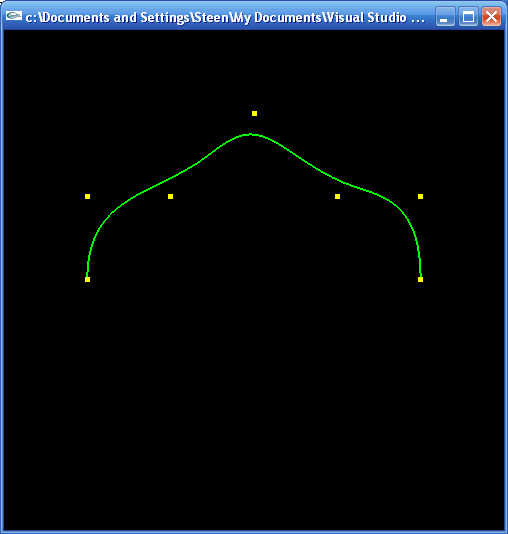
\includegraphics[width=8cm]{../exercise11/screenshots/1.png}
\caption{Kurve med kontrolpunkter}
\label{fig:11-1-1}
\end{figure}

\section{Part 2}

\texttt{Which type of surface is actually defined in the program?}

I bilaget til opgaven besvares sp�rgsm�let:

\begin{quote}
  The basis function is a cubic B-spline, but the knot sequence is
  nonuniform, with a multiplicity of 4 at each endpoint, causing the
  basis function to behave like a B�zier curve in each direction.
\end{quote}

\section{Part 3}

Resultatet ses i figur \ref{fig:11-3-1}.

\begin{figure}[hp]
\centering
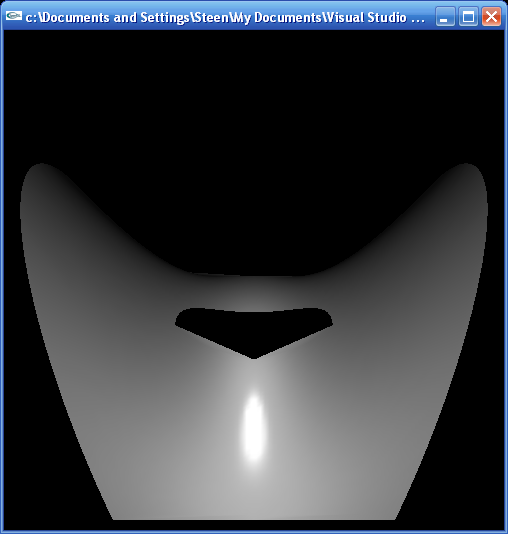
\includegraphics[width=8cm]{../exercise11/screenshots/3.png}
\caption{Et hul}
\label{fig:11-3-1}
\end{figure}